\documentclass{article}
%\usepackage[pdftex]{graphicx}
\usepackage{latexsym,epsf,epsfig}
\usepackage{amsmath,amsthm}


%    Q-circuit version 1.2
%    Copyright (C) 2004  Steve Flammia & Bryan Eastin, 4/23/06
%    This program is free software; you can redistribute it and/or modify
%    it under the terms of the GNU General Public License as published by
%    the Free Software Foundation; either version 2 of the License, or
%    (at your option) any later version.
%
%    This program is distributed in the hope that it will be useful,
%    but WITHOUT ANY WARRANTY; without even the implied warranty of
%    MERCHANTABILITY or FITNESS FOR A PARTICULAR PURPOSE.  See the
%    GNU General Public License for more details.
%
%    You should have received a copy of the GNU General Public License
%    along with this program; if not, write to the Free Software
%    Foundation, Inc., 59 Temple Place, Suite 330, Boston, MA  02111-1307  USA

\usepackage[matrix,frame,arrow]{xy}
\usepackage{amsmath}
\newcommand{\bra}[1]{\left\langle{#1}\right\vert}
\newcommand{\ket}[1]{\left\vert{#1}\right\rangle}
    % Defines Dirac notation.
\newcommand{\qw}[1][-1]{\ar @{-} [0,#1]}
    % Defines a wire that connects horizontally.  By default it connects to the object on the left of the current object.
    % WARNING: Wire commands must appear after the gate in any given entry.
\newcommand{\qwx}[1][-1]{\ar @{-} [#1,0]}
    % Defines a wire that connects vertically.  By default it connects to the object above the current object.
    % WARNING: Wire commands must appear after the gate in any given entry.
\newcommand{\cw}[1][-1]{\ar @{=} [0,#1]}
    % Defines a classical wire that connects horizontally.  By default it connects to the object on the left of the current object.
    % WARNING: Wire commands must appear after the gate in any given entry.
\newcommand{\cwx}[1][-1]{\ar @{=} [#1,0]}
    % Defines a classical wire that connects vertically.  By default it connects to the object above the current object.
    % WARNING: Wire commands must appear after the gate in any given entry.
\newcommand{\gate}[1]{*{\xy *+<.6em>{#1};p\save+LU;+RU **\dir{-}\restore\save+RU;+RD **\dir{-}\restore\save+RD;+LD **\dir{-}\restore\POS+LD;+LU **\dir{-}\endxy} \qw}
    % Boxes the argument, making a gate.
\newcommand{\meter}{\gate{\xy *!<0em,1.1em>h\cir<1.1em>{ur_dr},!U-<0em,.4em>;p+<.5em,.9em> **h\dir{-} \POS <-.6em,.4em> *{},<.6em,-.4em> *{} \endxy}}
    % Inserts a measurement meter.
\newcommand{\measure}[1]{*+[F-:<.9em>]{#1} \qw}
    % Inserts a measurement bubble with user defined text.
\newcommand{\measuretab}[1]{*{\xy *+<.6em>{#1};p\save+LU;+RU **\dir{-}\restore\save+RU;+RD **\dir{-}\restore\save+RD;+LD **\dir{-}\restore\save+LD;+LC-<.5em,0em> **\dir{-} \restore\POS+LU;+LC-<.5em,0em> **\dir{-} \endxy} \qw}
    % Inserts a measurement tab with user defined text.
\newcommand{\measureD}[1]{*{\xy*+=+<.5em>{\vphantom{\rule{0em}{.1em}#1}}*\cir{r_l};p\save*!R{#1} \restore\save+UC;+UC-<.5em,0em>*!R{\hphantom{#1}}+L **\dir{-} \restore\save+DC;+DC-<.5em,0em>*!R{\hphantom{#1}}+L **\dir{-} \restore\POS+UC-<.5em,0em>*!R{\hphantom{#1}}+L;+DC-<.5em,0em>*!R{\hphantom{#1}}+L **\dir{-} \endxy} \qw}
    % Inserts a D-shaped measurement gate with user defined text.
\newcommand{\multimeasure}[2]{*+<1em,.9em>{\hphantom{#2}} \qw \POS[0,0].[#1,0];p !C *{#2},p \drop\frm<.9em>{-}}
    % Draws a multiple qubit measurement bubble starting at the current position and spanning #1 additional gates below.
    % #2 gives the label for the gate.
    % You must use an argument of the same width as #2 in \ghost for the wires to connect properly on the lower lines.
\newcommand{\multimeasureD}[2]{*+<1em,.9em>{\hphantom{#2}}\save[0,0].[#1,0];p\save !C *{#2},p+LU+<0em,0em>;+RU+<-.8em,0em> **\dir{-}\restore\save +LD;+LU **\dir{-}\restore\save +LD;+RD-<.8em,0em> **\dir{-} \restore\save +RD+<0em,.8em>;+RU-<0em,.8em> **\dir{-} \restore \POS !UR*!UR{\cir<.9em>{r_d}};!DR*!DR{\cir<.9em>{d_l}}\restore \qw}
    % Draws a multiple qubit D-shaped measurement gate starting at the current position and spanning #1 additional gates below.
    % #2 gives the label for the gate.
    % You must use an argument of the same width as #2 in \ghost for the wires to connect properly on the lower lines.
\newcommand{\control}{*!<0em,.025em>-=-{\bullet}}
    % Inserts an unconnected control.
\newcommand{\controlo}{*-<.21em,.21em>{\xy *=<.59em>!<0em,-.02em>[o][F]{}\POS!C\endxy}}
    % Inserts a unconnected control-on-0.
\newcommand{\ctrl}[1]{\control \qwx[#1] \qw}
    % Inserts a control and connects it to the object #1 wires below.
\newcommand{\ctrlo}[1]{\controlo \qwx[#1] \qw}
    % Inserts a control-on-0 and connects it to the object #1 wires below.
\newcommand{\targ}{*!<0em,.019em>=<.79em,.68em>{\xy {<0em,0em>*{} \ar @{ - } +<.4em,0em> \ar @{ - } -<.4em,0em> \ar @{ - } +<0em,.36em> \ar @{ - } -<0em,.36em>},<0em,-.019em>*+<.8em>\frm{o}\endxy} \qw}
    % Inserts a CNOT target.
\newcommand{\qswap}{*=<0em>{\times} \qw}
    % Inserts half a swap gate. 
    % Must be connected to the other swap with \qwx.
\newcommand{\multigate}[2]{*+<1em,.9em>{\hphantom{#2}} \qw \POS[0,0].[#1,0];p !C *{#2},p \save+LU;+RU **\dir{-}\restore\save+RU;+RD **\dir{-}\restore\save+RD;+LD **\dir{-}\restore\save+LD;+LU **\dir{-}\restore}
    % Draws a multiple qubit gate starting at the current position and spanning #1 additional gates below.
    % #2 gives the label for the gate.
    % You must use an argument of the same width as #2 in \ghost for the wires to connect properly on the lower lines.
\newcommand{\ghost}[1]{*+<1em,.9em>{\hphantom{#1}} \qw}
    % Leaves space for \multigate on wires other than the one on which \multigate appears.  Without this command wires will cross your gate.
    % #1 should match the second argument in the corresponding \multigate. 
\newcommand{\push}[1]{*{#1}}
    % Inserts #1, overriding the default that causes entries to have zero size.  This command takes the place of a gate.
    % Like a gate, it must precede any wire commands.
    % \push is useful for forcing columns apart.
    % NOTE: It might be useful to know that a gate is about 1.3 times the height of its contents.  I.e. \gate{M} is 1.3em tall.
    % WARNING: \push must appear before any wire commands and may not appear in an entry with a gate or label.
\newcommand{\gategroup}[6]{\POS"#1,#2"."#3,#2"."#1,#4"."#3,#4"!C*+<#5>\frm{#6}}
    % Constructs a box or bracket enclosing the square block spanning rows #1-#3 and columns=#2-#4.
    % The block is given a margin #5/2, so #5 should be a valid length.
    % #6 can take the following arguments -- or . or _\} or ^\} or \{ or \} or _) or ^) or ( or ) where the first two options yield dashed and
    % dotted boxes respectively, and the last eight options yield bottom, top, left, and right braces of the curly or normal variety.
    % \gategroup can appear at the end of any gate entry, but it's good form to pick one of the corner gates.
    % BUG: \gategroup uses the four corner gates to determine the size of the bounding box.  Other gates may stick out of that box.  See \prop. 
\newcommand{\rstick}[1]{*!L!<-.5em,0em>=<0em>{#1}}
    % Centers the left side of #1 in the cell.  Intended for lining up wire labels.  Note that non-gates have default size zero.
\newcommand{\lstick}[1]{*!R!<.5em,0em>=<0em>{#1}}
    % Centers the right side of #1 in the cell.  Intended for lining up wire labels.  Note that non-gates have default size zero.
\newcommand{\ustick}[1]{*!D!<0em,-.5em>=<0em>{#1}}
    % Centers the bottom of #1 in the cell.  Intended for lining up wire labels.  Note that non-gates have default size zero.
\newcommand{\dstick}[1]{*!U!<0em,.5em>=<0em>{#1}}
    % Centers the top of #1 in the cell.  Intended for lining up wire labels.  Note that non-gates have default size zero.
\newcommand{\Qcircuit}[1][0em]{\xymatrix @*[o] @*=<#1>}
    % Defines \Qcircuit as an \xymatrix with entries of default size 0em.  The optional argument, #1, is for use with clusters, and allows you
    % to fix the size of the nodes.  I would not advise using it with normal circuits.
\newcommand{\node}[2][]{{\begin{array}{c} \ _{#1}\  \\ {#2} \\ \ \end{array}}\drop\frm{o} }
    % When Qcircuit has been passed the optional argument for cluster states, this command produces a round node of the size specified in that
    % argument.  The optional argument #2 specifies the contents of a node, while optional argument #1 is a secondary label.  
\newcommand{\link}[2]{\ar @{-} [#1,#2]}
    % Draws a wire or connecting line to the element #1 rows down and #2 columns forward.
\newcommand{\pureghost}[1]{*+<1em,.9em>{\hphantom{#1}}}
    % Same as \ghost except it omits the wire leading to the left. 
\xyoption{all}

\newcommand{\braket}[2]{\left \langle #1 \right. \left | #2 \right \rangle}

\title{Adiabatic Quantum Computers and Unsolvable Problems}
\author{Bill Davis\\Johns Hopkins University}
\date{December 9th 2008}

\begin{document}
\maketitle

\begin{abstract}
Quantum Computers exploit the peculiarities of the quantum world to out-perform classical electronic computers. This paper explores some of the wilder claims about adiabatic quantum computation and tries to understand if it can solve unsolvable problems. 
\end{abstract}

\tableofcontents

\pagebreak

\section{Introduction}
What makes Quantum Computers exciting? Certainly increased computational power, outside of the bounds of megahertz and transistor counts, is interesting. The development of quantum computers capable of manipulating as few as 100 qubits would be capable of cracking encryption codes that would take a classical computer longer then the lifetime of the universe.

But there are limits. While it may appear that quantum computation can offer exponential speed-up, this doesn't apply universally. Scott Aaronson puts it best: 
\begin{quotation}
Q: But couldn't quantum computers try all possible solutions in parallel, and thereby solve NP-complete problems in a heartbeat?

A: Yes, if the heart in question was beating exponentially slowly. \cite{aaronson} 
\end{quotation}

These limits certainly are not obvious, and to those who haven't studied in depth the quantum computational model, which includes the author up until several months ago, it seems that the speed-up achieved by quantum computers could be unbounded. Why can't quantum computers do computations in an infinite number of alternate universes and return the result to us moments later? I think the standard answer would be that, yes, quantum computers can do an exponential number of computations in a single clock cycle. This is easy to see immediately when considering the superposition created by a Hadamard gate. With n qubits and n Hadamard gates we can create a superposition with $2^n$ terms. But, we lose information contained in that superposition once a measurement is made, and in fact we lose everything except a single term. This is the crucial obstacle when confronting the obtainable speedup when developing quantum algorithms. In short quantum algorithms cannot solve NP-Complete problems in polynomial time. But what about unsolvable problems, can quantum computing help us there?

This question reduces to a more fundamental one. Are there computational limits which are as insurmountable as the speed of light? Most computer scientists would probably say that yes, there are limits to what we can compute. And in fact this limit may be somehow encoded as physical reality the same way mass and energy exist. However there are current theories that this is not the case. Kieu, in a number of papers, has put forth an algorithm which he claims can solve a non-solvable problem. There are a number of issues at play when trying to probe the limits of computability that require multi-disiplanary research. There are ties to computer science, electrical engineering, physics, quantum physics and astrophysics. Several of these aspects will be examined here, and framed within the context of quantum computers. 

First, what is the relationship between physical reality and computability? Does physical reality impose strict limits on what is computable? Can we even develop a theory in which the uncomputable things are computable? 

Second, does the formalism associated with quantum computation make a difference when it comes to computability? In particular, do Adiabatic Quantum Computers (AQC) offer additional speed-up over conventional quantum computing. What about claims that AQC can not only solve NP-Complete problems quickly, but can theoretically decide undecidable questions in a finite amount of time.  


\section{Classical Computability} 
In the 1930's Turing introduced the imaginary Turing machine and he along with Church eventually postulated that any function which we would consider to be computable, can be computed by a turning machine. For our purposes the chief limitation imposed by the notion of computability is that a function is computable only if the computation can happen in a finite amount of time. I think it's also interesting to tie Turing machines to reality. 
\begin{quotation}
It is widely acknowledged that every physical system corresponds to a computational process, and that every computational process, if applicable, has to be physically and operationally feasible in some concrete realization. \cite{leitsch-2007}
\end{quotation}
This is important because in considering quantum computation we are harnessing a concrete realization of a computational process. If we can prove, one way or the other, the relationship between NP-Complete problems and quantum computers, and further that P $\ne$ NP, we have then learned something about the fundamental nature of the universe. 



And we can extend this concept to include not just the relationship between P and NP but also the relationship between computable and non-computable functions. Very early on in the study of the field Turing was able to show that there existed problems which are unsolvable from the standpoint of a Turing machine. This along with Godel's Incompleteness Theorem effectively demonstrated the limits of mathematical thought. So, given that we know problems exist which we cannot solve, not even in principal, what is the advantage of further discussion. Do computers exist more powerful then Turing machines, so called hypercomputers. Even if they did what could we say about them?

For the purposes of this paper I will be considering a few instances of provably NP-Complete and non-decidable problems.  

\subparagraph{3SAT}
Satisfiability is the problem of determining whether a given Boolean sentence contains variable assignments such that the sentence evaluates to true. There is no known algorithm for this problem which is better than brute-force search through all the possible variable assignments. 3SAT is a special instance of SAT where each clause of the Boolean sentence contains 3 Boolean literals. An example sentence of this form is 
\[
(A \lor B \lor C)  \land (A \lor E \lor F)
\]
The general case of satisfiability can be reduced to 3SAT. This problem will come into play with the description of Adiabatic Quantum Computing because of its easy formulation as a particular Hamiltonian. 

\subparagraph{Hilbert's Tenth Problem}

\begin{quotation}
Given a Diophantine equation with any number of unknown quantities and with rational integral numerical coefficients:  To devise a process according to which it can be determined by a finite number of operations whether the equation is solvable in rational integers. 
\end{quotation}

In short is there a general algorithm which takes a input a Diophantine equation and produces as output either a set of integer assignments which solves the problem or outputs cannot be solved. A Diophantine equation is a polynomial with solutions restricted to the integers. This problem is of importance because in the 1970's it was proven that a general algorithm for solving Diophantine equations would require a search through an infinite set. As there is no way of determining whether this infinite search will find an answer or not, in finite time, this problem is undecidable. 

This problem is described because Kieu uses it due to its equivalency to the Halting problem. 

\section{Hypercomputation}

\begin{quotation}
To better understand the relationship between classical computation and hypercomputation, it is useful to consider the relationship between Euclidean and non-Euclidean geometry. \cite{Ord06themany}
\end{quotation} 

In order to understand if Adiabatic Quantum Computers can solve Unsolvable problem it might help to discuss what it even means to solvable an unsolvable problem. It certainly seems to defy logic to even consider the issue as non-Euclidean geometry might have seemed to early geometers. First it might help to clarify terminology. Kieu used the term noncomputable, and Hodges uses classically insolvable. Both of them are referring to perhaps a better term undecidable. But really they are referring to problems which cannot be decided using Turing Machines. The leap from undecidable over Turing machines to unsolvable in general follows from the Turing-Church hypothesis that in order for a problem to be solved, in a manner we might all agree is in fact correct, it must be computable by a Turing Machine. Then it follows that problems which cannot be solved using a Turing Machine cannot in fact be solved by any machine that can actually exist.  In order to lay the groundwork for this discussion, consider the following scenario, which might help to identify the relevant issues. 

Is it physically impossible to solve the Halting Problem? There have recentely been investigations into this question. One of the more interesting cases involved relativistic Turing machines. Take a Turing machine M and a program P, which may or may not halt given some input. Take the machine, programmed with P and set it running on a computer located within a spaceship. Take the spaceship and fire it toward a singularity, e.g. a black hole, with the computer programmed to fire a rocket if the program ever halts. Since the spaceship will experience an infinite amount of time relative to an outside observer, if the program ever completes, it will in fact fire the rocket in finite time relative to an outside observer. We will be able to see the rocket, or otherwise detect some result, in some finite amount of time \cite{stannett-2008}. However since the spaceship is inside a black hole the event will be undetactlable outside the influence of the black hole. This requires that, in order to use this relativistic computer or obtain the results of the calculation, any outside programmer will also have to be inside the event horizon of the black hole in order to detect the outcome of the computation. This is ok, however, because by finding a rotating Kerr black hole, any scientists who want to determine the consistency of the Zermelo-Frankel axioms will be able to lead full lives after they launch their computer, provided they never try to leave the confines of the black hole which they entered \cite{A_abstractrelativistic}. 

\begin{figure}
\begin{center}
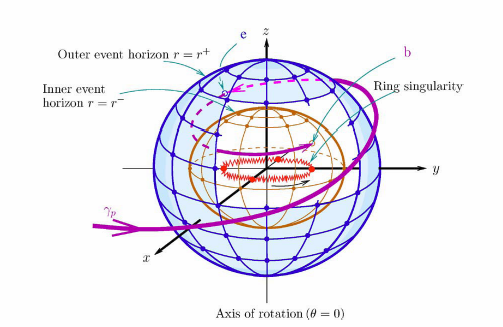
\includegraphics[height=70mm]{rotating3.png}
\caption{This illustration from \cite{A_abstractrelativistic} shows how a Kerr rotating black hole consisting of two event horizons and a singularity can support a relativistic Turing machine. }
\end{center}
\end{figure}

The study of machines which can perform computations above and beyond classical Turing machines is called Hypercomputing and there have been a number of very recent papers which have attempted to formalize the terms and definitions of this newly emerging field. There have been a number of extension proposed to classical Turing Machines including \cite{Ord06themany};
\begin{enumerate}
\item
 Oracles, or an unspecified device which can determine set membership.
\item 
Random Turing machines, where the Turing machine has access to a random bitstrings.
\item 
Infinite Time machines, Zeno Turing machines, where each computational steps takes half the time as the one before it.
\item Turing machines with an infinite input or infinite number of states.
\end{enumerate} 
Some of these extensions allow the machine to compute more then what a standard Turing machine is capable of. The physical manifestation of one of these machines while certainly unlikely is hopefully not impossible. 

This shows that extensions to Turing machines are a valid field of study. Developments in this inter-disciplary field will drive understanding of the physical limitations imposed upon computational power. 



\section{Adiabatic Quantum Computation}
Adiabatic Quantum Computation (AQC) is an attempt to create another model of computation that incorporates quantum physics but does not use the standard model of quantum gates implemented by unitary operators. It instead based upon the adiabatic theorem of quantum physics which states formally that if there exists a quantum system with Hamiltonian $H_1$ with ground energy state $\Psi_1$ and we transform the system into $H_2$, using the transformation 
\[
H \frac{t}{T} = (1-\frac{t}{T})H_1+\frac{t}{T}H_2
\]
then the ground energy state $\Psi_1$ is transformed into $\Psi_2$ where $\Psi_2$ is the ground energy state of the system $H_2$ \cite{kieu-2003-44,ambainis-2004}. This process takes place over time $T$. An immediate question one might have is what is the value of T. Since the total time T directly relates to the runtime of the process, how can we know that T can be controlled when solving computational problems? While full discussion of this appears in a later section here we can say that there really isn't enough empirical evidence at this time to fully describe how T can be controlled. It will even be different from one problem to another and even differ based on the parameters used when solving a problem. 

AQC uses this trick of quantum mechanics as a model of information in the following way. A system is purposefully put into known ground state with Hamiltonian $H_1$. The answer to some problem is encoded into a Hamiltonian $H_2$, for which the ground state may not be able to be calculated. The system is then transformed, according to the adiabatic theorem, into a system with Hamiltonian $H_2$. The adiabatic theorem then guarantees that the system will then be in state $\Psi_2$, which is the answer to our problem. This is true even when $H_2$ has any number of possible energy states/eigenvalues. By measuring the system and obtaining the value for $\Psi_2$ we have answered the question we set out to solve. 

What makes this a useful model for computation was put forward in \cite{farhi-2000} 

\begin{quotation}
Many computationally interesting problems can be recast into an equivalent problem of finding a variable assignment that minimizes an "energy" function. 
\end{quotation}

\cite{farhi-2000} apply AQC to 3SAT in the following manner. For a boolean statement with anynumber of clauses $C$, each with 3 variables $i_C, j_C, k_C$, define an energy function 
\begin{equation*}
h_C(i_C, j_C, k_C)= 
\begin{cases} 0 & \text{if the clause is satisfied by ($i_C, j_C, k_C$)}
\\
1 &\text{Otherwise}
\end{cases}
\end{equation*}
The total energy of the system is then the sum of the energies of each clause in the statement. 
\[
h = \sum_{C}h_C
\]
By minimizing the energy of this equation $h$ we can find if any Boolean statement has a satisfying assignment. This can be found by locating the ground energy state of a system with Hamiltonian $H_p$ where
\[
H_p = \sum_cH_{P,C}
\]
Each $H_{P,C}$ represents an encoding of a Boolean clause in the Hilbert space spanned by $N= 2^{N}$ basis vector where $N$ is the number of qubits used in solving the problem. This feature of the algorithm is similar to the standard model of quantum computation. That is, a Boolean statement with $N$ variables can be encoded into a Hamiltonian with $N$ qubits, with a space spanned by $2^N$ basis vectors. If we could calculate the ground state of $H_p$, then we would be able to determine if the Boolean clause is satisfiable, or not. 

The chief difference, then, between this AQC model and the standard quantum computational model is the area of measurement. In the standard model the exponential state space is usually in a superposition, and any measurement instantaneously forces the system into an eigenvector based upon a probabilistic assignment. There is no way to determine from the measurement what the state of the system was the moment the measurement was made. With AQC, a measurement is made when the system is in a state described by the Hamiltonian $H_2$, and because the system was in the ground state $\Psi_1$ when the process was started the system is guaranteed to by in the ground state $\Psi_2$ when the process is over. Therefore the measurement should always be happening on a system which is \emph{always} in an eigenstate, and not in a superposition of states.

\subsection{Constructability of AQC Machines}
There have been a number of claims related to the benefits of AQC over the standard quantum computing model. Without more research it will be difficult to tell the hype from the reality for some time. 

One of the potential advantages of AQC is the ease with which quantum computers based on this model can be built. It appears that quantum circuits of the nature can be built using today's technology on something resembling silicon circuits. In 2007 \cite{vanderploeg-2007} were able to create a three qubit system using flux qubits.  


\begin{figure}
\begin{center}
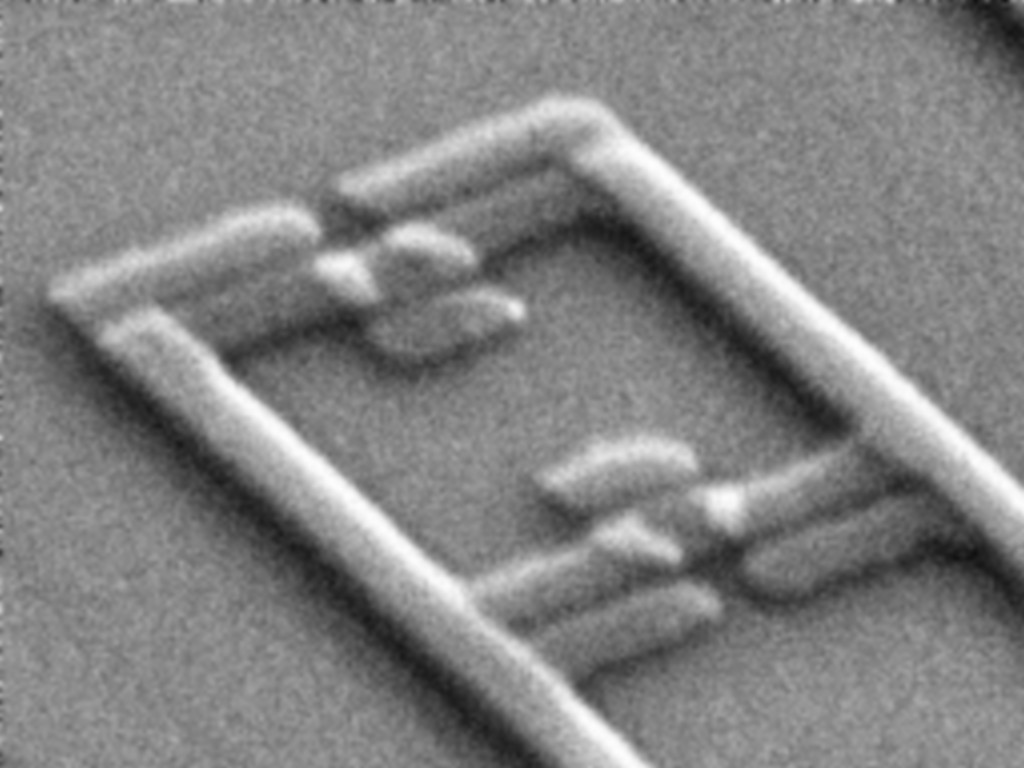
\includegraphics{5261025.jpg}
\caption{An Electron Microscope image of a flux qubit. These qubits are generated using a voltage source and a resonator tank-circuit for readout of results}
\end{center}
\end{figure}

The physical operation of these quantum systems is well beyond the scope of this paper. But in principal a AQC based computer can operate by electrical principals. "By applying a dc bias current through the tank and currents through the lines we can separately change the magnetic flux in the qubits." \cite{vanderploeg-2007}. This flux manipulation allows the computer to manipulate the Hamiltonian of the system, effecting the adiabatic change. 

There is even a commercial company, D-Wave, which claims to have constructed a multi-qubit system based on this principal. They have issued press releases like "World's First Commercial Quantum Computer Demonstrated" and "World's First 28-qubit Quantum Computer Demonstrated Online at Supercomputing 2007 Conference". These claims seem more marketing speak then actual progress, no one has independently verified that they are producing entangled qubits but it is likely they are close to demonstrating a working quantum computer with multiple qubits. One of the principal problems faced with when constructing working machines is that in order to obtain the initial ground state, the quantum computer, or at least the pieces one would like to operate adiabatically, must be cooled almost to absolute zero degrees. To solve this problem D-Wave "cools circuits made of the rare metal niobium to five-thousandths of a degree above absolute zero." \cite{discoveryMag}

But even if AQC machines are actually constructed, what kind of performance advantage will they be able to obtain? Current evidence in this regards is somewhat mixed, due to the uncertain nature of the AQC process and what reasonable expectations are for their performance. 


\subsection{The Spectral Gap}

One of the interesting results developed as a consequence of AQC is the relationship between the spectral gap and computational complexity. The spectral gap is directly related to the amount of time T required to a process to be performed adiabatically. This time was directly calculated in \cite{vandam-2002} as 
\[
\tau(s) \gg \frac{ \frac{d H(s)}{ds}}{g(s)^2}
\]
where g(s) denotes the gap between the smallest eigenvalues of H(s), in other words the energy gap between the ground state and the first energy state. It follows that the larger this gap is, the faster the adiabatic process can be. So what determines the size of this gap?

As it turns out, the gap size may be related to the computational difficulty of the problem. In \cite{mitchell-2008}, simulated experiments were run using AQC solve different instantiations of 3SAT. 3SAT problems can be described by the relative difficulty as function of the ratio between clauses and variables. \cite{mitchell-2008} developed a

\begin{quotation}
correlation between quantum spectral complexity and 'classical' computation complexity and the formulation of a quantitative correspondence between the two systems.
\end{quotation}

The implication of this is that like heuristic techniques, there may be cases where an ACQ algorithm performance will differ drastically as a function of the input. Increased computational complexity could lead to increased spectral complexity which in turn increases the time needed for a the adiabatic process. 

\subsection{Kieu and Noncomputability}
The chief proponent of claims that AQC can solve NP-Complete and Turing non-decidable problems is Tien Kieu from Swinburne University of Technology in Australia. Kieu presents a general algorithm which he claims is capable of deciding whether an arbitrary Diophantine equation has a solution or not. What follows is a brief summarization of his algorithm. For more details consult \cite{kieu-2006-2,kieu-2003-44,kieu-2005,kieu-2003-5105,kieu-2006-3}. The first step is to develop a Hamiltonian representation $H_p$ of the Diophantine equation under consideration and then eventually use AQC to evolve a known ground state $H$ into $H_p$. This translation is canonical, for a given Diophantine equation $D(x_1,x_2 ... x_K)=0$ with K variables,

\[
H_p = (D(a_1^\dag a_1 ... a_K^\dag a_K))^2
\]

Where $a$ and $a^\dag$ are the creation and annihilation operators for the Fock space. And the operator $a_1^\dag a_1$ is the number operator which gives the particular number of particles in a specific state. Specifically  
\[
a = \left(\begin{array}{cccccc} 
0 & \sqrt{1} & 0 & 0 & ...\\ 
0 & 0 & \sqrt{2} & 0 & ...\\ 
0 & 0 & 0 & \sqrt{3} & ... \\
0 & 0 & 0 & 0 & ...
\end{array}\right)
\]

This is one important difference between Kieu's treatment of AQC and the standard model of quantum computation. Kieu requires that the infinite dimensional Hamiltonians exist in a Fock space, which is a kind of Hilbert space with a variable number of basis vectors. In normal quantum computation, qubits exist in spaces with $2^N$ basis vectors when operating on $N$ qubits. To realize Kieu's process requires implementing a physical system having an infinite number of energy levels. 

The other important variable defined is the initial Hamiltonian for the system,
\[
H_I = \sum^K_{i=1} (a_i^\dag - \alpha_i^*)(a_i-\alpha_i)
\]
for some complex number $\alpha$

The last variable which needs to be assigned in order for the AQC to perform its magic is the value T, which is the length of time over which the algorithm needs to operate. There is a problem here, however. In this case we do not "in advance know in general how long is sufficiently long" for the transformation to occur, so we do not know what to set the value T too. Tieu fixes this up by showing that we can probabilistically identify the ground state. 
\[
\ket{n_0} \text{is the ground state of } H_p \Leftrightarrow |\braket{\psi{T}}{n_0}|^2 > \frac{1}{2}
\]
That is, after evolving the system for some time T, we perform a number of measurements, and we obtain one state with probability more then 0.5, we know that state is the ground state and we're done. Otherwise we continue to increase T, until we obtain our result. Kieu asserts that he has shown that "we can confidently know that for each Diophantine equation and each set of $\alpha$'s, there is a \emph{finite} evolution time after which the adiabaticity condition is satisfied." 

So here is the algorithm.
\begin{enumerate}
\item 
Put the system into the ground state with Hamiltonian $H_i$, which is a "well known coherent state in quantum optics" \cite{kieu-2005}.
\item Evolve the system for some time T
\item Make K measurements of the system obtaining states $\ket{k_i}$. 
\item If any $\ket{k_i}$ happens when frequency greater than $\frac{K}{2}$ we are ready to return a solution. If not, return to step 2. 

\end{enumerate} 


\section{Objections to AQC Hypercomputability}
As might be expected with such a controversial claim, there have been numerous objections leveled against Kieu's ideas. To be fair, he has subsequently attempted to address every objection brought to bear on AQC hypercomputability. The objections can be divided into two categories, technical and theoretical. The technical objections are hard to decipher for an outsider to quantum theory. They involve the specifics of the Hamiltonian used to encode the Diophantine equation as well as the mechanics of the time evolution process as it interacts with the spectral gaps between energy states. The theoretical objections revolve around the dynamics of information theory and the possibility of infinite search in finite time or the equivalency between AQC and the standard model of quantum computation. 

\subsection{Probabalistic Nature} 
Since the value of total time T for adiabatic transformation is unknown when the algorithm is started, it is necessary to probabilistically determine when the algorithm is terminated. After T time has elapsed and 100 measurements are made, a non-ground state measurement may be obtained 51 times. Since this triggers the termination criteria, the algorithm will have returned an incorrect result. Kieu addresses this by appealing to the Weak Law of Large Numbers, by noting that the error is inversely proportional to the number of samples taken. Therefore error can always be made as small as possible by taking a sufficient number of samples. 

\subsection{AQC is equivalent to the Standard Model of Quantum Computation}
It was shown in \cite{aharonov-2007-37} that the adiabatic computation model and the standard model of quantum computation involving unitary gates are polynomial equivalent. What is the effect upon Hypercomputation using AQC. At first it would appear to severely limit the possibilities. We know, for example, that we can simulate quantum computation using a regular digital computer. It follows that a digital computer and a quantum machine can calculate the same things. If AQC and the standard model are polynomial equivalent, then whatever it calculable by AQC is also calculable by a run of the mill digital computer. 

Kieu responds to this by invoking the infiniteness of the Fock space in which the calculations take place as opposed to the finite Hamiltonians used in the standard formalisms. Kieu's approach

\begin{quotation}
%We can only offer here some speculations about this apparent
%discrepancy
%The quantum Turing machine approach is a direct generalisation of that of the
%classical Turing machines but with qubits and some universal set of one-qubit and two-qubit
%unitary gates to build up, step by step, dimensionally larger, but still dimensionally finite
%unitary operations. This universal set is chosen on its ability to evaluate any desirable
%classical logic function.
%Our approach, 
... is from the start based on
infinite-dimension Hamiltonians acting on some Fock space and also based on the special
properties and unique status of their ground states. The unitary operations are then
followed as the Schr�odinger time evolutions. Even at the Hamiltonian level higher orders
of the operators a and a�, i.e. not just two-body but many-body interactions in a sense,
are already present. This proliferation, which is even more pronounced at the level of
the time-evolution operators, together with the infinite dimensionality and the unique
energetic status of the vacuum could be the reasons behind the ability to compute, in a
finite number of steps, what the dimensionally finite unitary operators of the standard
quantum Turing computation cannot do in a finite number of steps \cite{kieu-2003-44}.
\end{quotation}

Is this claim convincing? It seems that Kieu has simply replaced an infinite time calculation with an infinite Fock space. The question then seems to become can this Fock space, in practice, be realized in the physical world. This definitely limits the applicability of the algorithm because even Kieu admits, 

\begin{quotation}
we cannot have available an unbounded number of levels for the quantum algorithm  \cite{kieu-2003-44}.
\end{quotation}

Is this limitation similar in nature to the finiteness of memory used in a Turing machine. After all there are physical limitations on how much memory can be in use by a Turing machine, despite in the infinite ideal. This question likely deserves more research and is seems to be tied to the amount of information that can be physically realized in a single location. \footnote{As Kieu has a point to every counter-point, he notes that a "finitely prepared qubit can have infinite algorithmic informational theoretic complexity" \cite{kieu-2005}. This can be achieved by alternating non-compatible observables to generate a (truly) random sequence of bits. }


\subsection{Infinite Precision}
There are a number of issues that come into play when considering the effect that precision will have on Kieu's algorithm. First, what will happen when a discrete set, the integers, is translated into a Hamiltonian which has members that take on real values. As Hodges notes \cite{hodges-2005}, if we try translating the value 2 and end up with 2.0000... any error would "wreck" the results of the calculation. Kieu addresses this issue directly, describing the distinction between infinite precision and unbounded precision. While Hodges and other critics claim that infinite precision is required in order to realize the algorithm, Kieu has the opinion
\begin{quotation}
that it may not be a foregone conclusion, as some may have thought, that the physically available precision is not adequate for an implementation of the proposed algorithm.
\end{quotation}
Here unbounded refers to as much precision as the implementer has the time or desire to achieve. This is certainly not an extremely convincing argument. Kieu also tries to resolve this difficulty with multiple samples, achieving a statistical average inversely proportional to $\sqrt{N}$ for $N$ trials. Increasing N until "we could confidently confirm the (integer-valued) central value."

Along with precision comes the introduction of noise. Since these quantum systems must be kept in the ground states for the Adiabatic transition to occur, it seems that they can be extremely susceptible to environmental noise. Kieu claims that even "though
these fluctuations in the energy levels are ever present and cannot be reduced to zero, there
is no physical principle, and hence no physical reason, why their size cannot be reduced to
a size smaller than some required scale." What is left to be understood is how the effect of an infinite number of energy states can be managed so that the spectral gap is large enough to allow the algorithm to succeed. And additional work by \cite{mitchell-2008} seems to indicate the computational complexity and spectral gaps are inextricably linked. 

\subsection{The existence of decoy ground states}
Smith in \cite{Smith05d2006} produced a strong critique of Kieu's algorithm, attempting to show that there were situations in which the system undergoing the Adiabatic change failed to stay in the ground state. These situations which he labeled as decoy ground states appear to occur frequently. Smith claimed in every 25 simulations, 1 produced a decoy ground state. Kieu claims in \cite{kieu-2005} that no matter what the value of T, there will never be a situation where the probability of measuring a non-ground state is greater the $\frac{1}{2}$. This is different than the first argument about the probabilistic nature of the algorithm. There, non-ground states may appear to be measured with frequency greater than $\frac{1}{2}$, but this is nothing more than a statistical aberration which will likely disappear with an increasing number of samples. 

In detail, Smith chose of $H_1$ and $H_p$ values, 

\[
H_1 = \left(\begin{array}{ccccc} 
1 & -1 & 0 & 0 & 0 \\
-1 & 2 & - \sqrt{2} & 0 & 0 \\
0 & -\sqrt{2} & 3 & -\sqrt{3} & 0 \\
0 & 0 & -\sqrt{3} & 4 & -\sqrt{4} \\
0 & 0 & 0 & -\sqrt{4} & 5 \\
\end{array}\right)
, 
H_p = \left(\begin{array}{ccccc} 
2 & 0 & 0 & 0 & 0\\
0 & 4 & 0 & 0 & 0 \\
0 & 0 & 5 & 0 & 0\\
0 & 0 & 0 & 3 & 0\\
0 & 0 & 0 & 0 & 1
\end{array}\right)
\]
Which is an application of Kieu's algorithm for a Diophantine equation with 1 variable and setting $\alpha$ to 1. After evolving the system for T=13.344 the system has eigenvalues 
\[
0.0144,1.1307,2.5406,4.3884,6.9288
\]
Which occur with probabality 
\[
0.0139,0.9997,0.0062,0.0210,0.0015
\]
Here the second energy level 1.1307 has a .9997 percent chance of being measured, and returning a wrong value from the algorithm. 

Kieu has a response to this, although it is not entirely satisfying. Since this numerical simulation is required to take place on a real machine, an infinite Fock space cannot be simulated, and Smith chose to truncate the Hamiltonian to 5 basis vectors. Kieu again appeals to the infinite Fock space claiming that, 

\begin{quotation}
In general, we suspect that the possibility of the violation [noted by Smith] \emph{is an artifact of the truncation of the Fock space} since it is extremely sensitive to the truncation and associated boundary conditions \cite{kieu-2006-3}.
\end{quotation}



\subsection{Infinite Search In Finite Time}

Grover's search algorithm gives a $\sqrt{N}$ speedup of unstructured search problems. Isn't it the case that Kieu's algorithm beats that by searching an infinite number of integers for one which satisfies the Diophantine Equation? Kieu responds to this with the argument that finding the solution to a Diophantine equation is a finitely refutable problem. That is, if no solution exists, \emph{within a finite domain} then there is no solution anywhere. Due to the physical nature of the encoding used for the AQC, the adiabatic process somehow "knows" what the finite domain is, based upon ground states available to it. 

For example, classical minimization algorithms are unable to distinguish between a global minimum and a local minimum. Minimization algorithms based upon AQC in fact can distinguish between local and global minimum. This fact follows from that Kieu claims, as above, that there are no level crossings in the spectral flow between \emph{any} pair of eigenstates. This allows Kieu's to ultimately reduce to finite search. This selection of an finite domain from an infinite one seems to be a bit magical. It also seems unclear why we are unable to locate this finite domain outside the bounds of quantum mechanics, that is, what exactly is encoded in the nature of the algorithm that allows for this selection, and how can we know its correctness. 

\section{Conclusion}
Can AQC compute answers to Turing non-decidable questions, absolutely. Will this computation happen in a finite time, probably. Will the answer computed be correct, probably not. It seems that there are too many physical and theoretical limitations in order to realize the fantastic claims of Kieu with regards to Diophantine equations. It is still an open question of whether or not the universe is constructed in such a way as to prevent Turing non-decidable questions from ever being answered, at least without taking a rocket ship into a black hole. Kieu has addressed, and re-addressed many issues and all complaints against his algorithm but cannot make some of his fundamental assumptions disappear. There seems to be a lot of smoke but only a little fire. Particularly unconvincing is the failure to resolve the number of energy levels required for the algorithm to operate. It seems unclear if physical systems can be generated, without a infinite amount of energy, that are able to be in an infinite number of possible eigenstates. Without operating in this infinite space, the algorithm reduces to a truncated version with a finite number of basis vectors and this case was provably shown to produce decoy ground states. 

On the other hand AQC seems like it does have a lot to offer over the standard model of quantum computation and represents an extremely promising approach to quantum computing. Perhaps its future lies along the same path as some artificial intelligence techniques like neural nets and simulated annealing. These techniques can be extremely useful applied to certain kinds of problems with certain kinds of input, where approximation is acceptable. They currently represent the state of the art when it comes to "solving" NP-Complete problems. They may not give the correct answer 100\% of the time, but at least they give \emph{an} answer in polynomial time. If AQC can be shown to have applicability to difficult problems, and outperform other AI techniques, then it wouldn't be surprising to see special purpose AQC machines built that can act as a probabilistic oracle to regular digital computers. Their answers will have to be verified, however it may be possible to generate results with an extremely high degree of accuracy to otherwise intractable problems. 




\bibliography{Paper}
\bibliographystyle{amsalpha}
\end{document}
